\documentclass[12pt]{book}
\usepackage[a4paper,bindingoffset=0.2in,%
            left=0.75in,right=0.75in,top=1in,bottom=1in,%
            footskip=.25in]{geometry}
\usepackage{fancyhdr}
\setlength{\headheight}{15.2pt}
\usepackage[utf8]{inputenc}
\pagestyle{fancy}

\renewcommand{\chaptermark}[1]{\markboth{\thechapter.\ #1}{}}
\renewcommand{\sectionmark}[1]{\markright{\thesection\ #1}}
\fancyhead[LE,RO]{\textbf{\thepage}}
\fancyhead[LO]{\textbf{\rightmark}}
\fancyhead[RE]{\textbf{\leftmark}}
\fancyfoot{}
\fancypagestyle{plain}
{
    \fancyhf{}
}


\usepackage{amsmath}
\usepackage{amssymb}
\usepackage{mathtools}
\usepackage{xcolor}
\usepackage{enumitem}
\usepackage[ruled,noline]{algorithm2e}
\usepackage{graphicx}
\usepackage{common}
\usepackage{english-theorems}
\setcounter{tocdepth}{1}

\begin{document}
\tableofcontents
\clearpage
\ifodd\value{page}\else
\thispagestyle{empty}
\fi
\chapter{Kernel Abstraction}

\section{The process concept}
\chapter{Slides}
\section{Lecture 1}
The key building blocks of OS
\begin{itemize}
    \item Process 
    \item Threads, Concurrency, Scheduling, Coordination
    \item Address space
    \item Protection, Isolation, Sharing , Security
    \item Communication, Protocols
    \item Persistent storage, Transaction, Consistency, Resilience
    \item Interfaces all devices
\end{itemize}

\begin{figure}
    \centering
    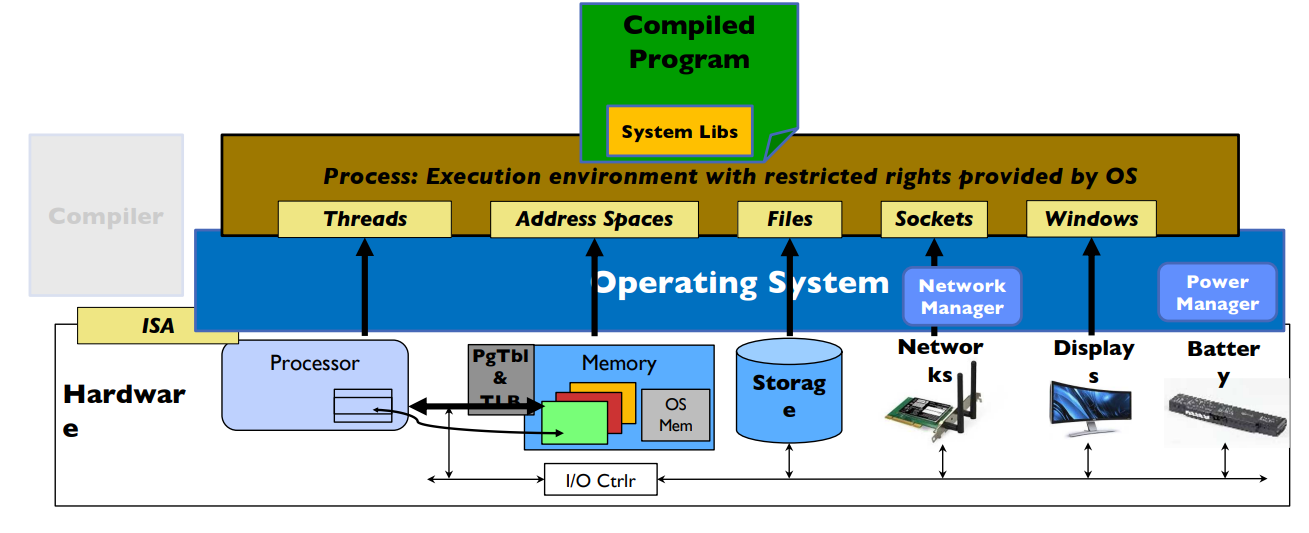
\includegraphics[width = 0.9\textwidth]{Chapters/graphics/OSAbstraction.png}
\end{figure}

\section{Lecture 2}
\subsection{Thread}
A single unit execution context 
\begin{itemize}
    \item It has program counter (PC), registers, execution flags, stack, and memory state
    \item A thread executes on a processor when it is \underline{resident} in the processor's register.
    \item A thread is suspended when its state is not load into processor.
    \item When a thread is not running it's saved in the memory called \underline{thread control unit (TCB)}. 
    \item TCB is saved in kernel.
\end{itemize}

\subsection{Address space}
The set of accessible address and the state associated with them.

\subsection{}
An operating system must 
\begin{itemize}
    \item protect itself from user programs.
    \item be reliable.
    \item be secure.
    \item ensure privacy.
    \item ensure fairness.
    \item protect programs from one another.
    \item prevent threads owned by one program to impact other
\end{itemize}
\subsection{Simple protection: Base and Bound (B\&B)}
sets lower and upperbound for a program to access.

\subsection{Process}
execution enviroment with restricted access. 
\begin{itemize}
    \item (Protected) address space with one or more threads
    \item owns memory
    \item has file descriptors, file system context
    \item encapsulate one or more therad sharing process resources.
\end{itemize}

\subsection{Dual mode}
\begin{enumerate}
    \item Kernel mode (superivor)
    \item User mode
\end{enumerate}

\section{Lecture 3}
\subsection{Motivation for threads}
Operating system needs to handle multiple things at once.
\begin{description}
    \item[Multiprocessing:] multiple CPU.
    \item[Multiprogramming:] multiple jobs/processes.
    \item[Multithreading:] multiple threads.   
\end{description}
Threads are mainly in three states 
\begin{enumerate}
    \item Running: running.
    \item Ready: eligible to run.
    \item Blocked: ineligible to run.
\end{enumerate}

\subsection{pthreads API}
\begin{description}
    \item[pthread\_create]
    \item[pthread\_exit] 
    \item[pthread\_join] suspends the execution calling thread until the target thread terminates.  
\end{description}

to avoid race conditions
\begin{itemize}
    \item Mutual exclusion: ensuring only one thread does a particular thing at a time.
    \item Critical sections: code exactly one thread can execute at a time.
\end{itemize}

\subsubsection*{Locks}
\begin{description}
    \item[acquire:] wait until lock is free.
    \item[release:] mark lock as free.  
\end{description}
both these operations are atomic. and done with pthread\_mutex\_init,lock,unlock.

\subsubsection*{Process}
Bootstrapping: every process is created from another process. first process is started by the kernel and is often called the init process.

\begin{description}
    \item[exit:] exits a process.
    \item[fork:] creates a brand new process and copies the whole process image.
    \item[exec:] changes the program being run.
    \item[wait:] wait for a process to finish.
    \item[kill:] send a signal to another process.
    \item[sigaction:] set handlers for signals.      
\end{description}

\section{Lecture 4}
\subsection{Semaphores}
Semaphores are non-negative integers.
\begin{description}
    \item[P()/down():]  atomic operation that waits for the semaphore to become positive, then decrement it by one.
    \item[V()/up():] atomic operation that increments semaphore by one, waking up a waiting process if any. 
\end{description}
\subsection{File system abstraction}
\begin{description}
    \item[File:] collection of data in a file system. 
    \item[Directory:] Hierarchical naming, links, volumes. 
\end{description}
every process has a current working directory.

\begin{description}
    \item[Absolute path:] /home/.
    \item[Relative path:] ../ for parent, ./ for current, ~/ for absolute path and a function of shell.  
\end{description}

\subsection{High level file API- Streams}
files are treated as unformated sequence of bytes.
FILE* fopen(,)

Key UNIX I/O design concepts 
\begin{itemize}
    \item Uniformity: everything is a file.
    \item Open before use
    \item Byte oriented
    \item Kernell buffered reads and writes
    \item Explicit close
\end{itemize}
open, creat, close,
int open() returns a file descriptor. open file descriptos are in kernel.
\subsubsection{Operation specific to terminals, devices, networking}
\begin{enumerate}
    \item ioctl()
    \item dup(), dup2()
    \item pipe()
    \item file locking
    \item memory mapping files
\end{enumerate}

\section{Lecture 5}
\subsection{Interprocess Communication (IPC)}
Communication between two or more processes. One way; data written by process A is held in memory until B reads it.
\subsubsection{UNIX pipe}
A writes to pipe, B reads from pipe.
\begin{itemize}
    \item If producer tries to write when buffer is full; it blocks.
    \item If consumer tries to read when buffer is empty; it blocks.
\end{itemize}
int pip(int fileds[2]);
\begin{itemize}
    \item allocates two new file descriptors in the process.
    \item writes to fileds[1] and reads from fileds[0].
    \item Implemented as fixed size queue inside kernel memory.
    \item After read file descriptor closes, writes generates SIGPIPE. If process ignores, then the write fails with an EPIPE error.
    \item After write file descriptor closes, pipe is effectively closed and reads return EOF.
\end{itemize}

A protocol is an agreement on how to communicate. which covers syntax and semantics.
Client server protocols: Cross network IPC.
Client initiates contact and server responses.
key idea: communication looks like file I/O.
\end{document}